\documentclass[12pt]{article}
\usepackage{polski}
\usepackage[utf8]{inputenc}
\usepackage{amsfonts}
\usepackage{amsmath}
\usepackage{enumitem}
\usepackage{graphicx}
\usepackage{float}
\usepackage{centernot}
\setlength{\parskip}{1em}

\usepackage{listings}
\usepackage{color} %red, green, blue, yellow, cyan, magenta, black, white
\definecolor{mygreen}{RGB}{28,172,0} % color values Red, Green, Blue
\definecolor{mylilas}{RGB}{170,55,241}

\lstset{language=Matlab,%
	%basicstyle=\color{red},
	breaklines=true,%
	morekeywords={matlab2tikz},
	keywordstyle=\color{blue},%
	morekeywords=[2]{1}, keywordstyle=[2]{\color{black}},
	identifierstyle=\color{black},%
	stringstyle=\color{mylilas},
	commentstyle=\color{mygreen},%
	showstringspaces=false,%without this there will be a symbol in the places where there is a space
	numbers=left,%
	numberstyle={\tiny \color{black}},% size of the numbers
	numbersep=9pt, % this defines how far the numbers are from the text
	emph=[1]{for,end,break},emphstyle=[1]\color{red}, %some words to emphasise
	%emph=[2]{word1,word2}, emphstyle=[2]{style},    
}


\begin{document}
	\title{Sprawozdanie\\Metody Numeryczne 2, laboratorium 3}
	\author{Grzegorz Rozdzialik (D4, grupa lab. 2)}
	\maketitle	
	
	\section{Zadanie}
	{\Large Temat \textbf{3}, zadanie \textbf{33}:}\\
	Obliczanie całek\
	$$\iint_D f(x, y) \,dx\,dy$$
	na obszarze
	$$D = \{(x, y) \in \mathbb{R}^2: |x| + |y| \leq 1\}$$
	przez podział $D$ na $4n^2$ trójkątów przystających, i zastosowanie na każdym z nich kwadratury rzędu 4-go.
	
	Obszar $D$ został przedstawiony na rysunku nr \ref{D-area}, jest to romb o środku $P_0 = (0, 0)$ i wierzchołkach
	\begin{align*}
		P_1 & = (1, 0)  \\
		P_2 & = (0, 1)  \\
		P_3 & = (-1, 0) \\
		P_4 & = (0, -1)
	\end{align*}
	
	\begin{figure}[H]
		\centering
		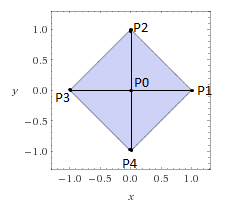
\includegraphics[scale=1.5]{images/D-area.png}
		\caption{Obszar $D$}
		\label{D-area}
	\end{figure}

	
	\section{Opis metody}
	\subsection{Podział rombu na $4n^2$ trójkątów}
	W celu podzielenia obszaru $D$ na $4n^2$ trójkątów użyto podział na 4 ćwiartki $D_1, D_2, D_3, D_4$ na podstawie osi układu współrzędnych. Podział ten został przedstawiony na rysunku nr \ref{D-quarters}.
	
	\begin{figure}[H]
		\centering
		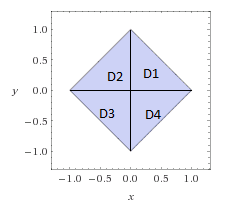
\includegraphics[scale=1.5]{images/D-quarters.png}
		\caption{Podział $D$ na ćwiartki}
		\label{D-quarters}
	\end{figure}

	Następnie każdą z ćwiartek podzielono na $n^2$ trójkątów według następującej reguły:
	\begin{enumerate}
		\item Każdy bok podzielono na $n$ równych części (punkty podziału nazwijmy węzłami).
		\item Węzły leżące na dwóch różnych bokach trójkąta i równoodległe od trzeciego z boków łączymy prostymi. Proste te będą wtedy równoległe do jednego z boków.
	\end{enumerate}

	Przykładowy schemat podziału ćwiartki $D_1$ z $n = 3$ ($D_1$ podzielono na 9 trójkątów przystających) został umieszczony na rysunku nr \ref{triangle-division}.
	
	\begin{figure}[H]
		\centering
		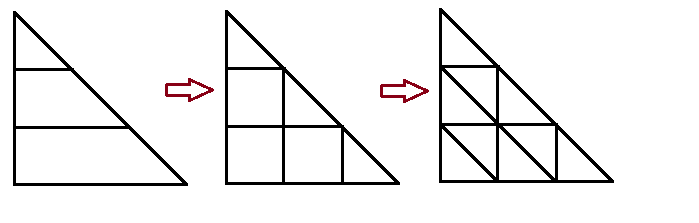
\includegraphics[]{images/triangle-division.png}
		\caption{Podział $D_1$ na 9 (= $3^2$) trójkątów}
		\label{triangle-division}
	\end{figure}

	Wszystkie $n^2$ trójkątów po podziale mają takie samo pole, równe $p = \frac{P}{n^2}$, gdzie $P = |D_1| = |D_2| = |D_3| = |D_4|$.
	
	Na każdym z tych trójkątów obliczamy wartość kwadratury 4-go rzędu:
	\begin{align}
		S(f) = & \frac{p}{60} \Bigg[  27f(P_{012}) + 3 \Big( f(P_{01}) + f(P_{02}) + f(P_{12}) \Big)  \nonumber \\
		       & + 8\Big( f(P_0) + f(P_1) + f(P_2) \Big) \Bigg] \label{kwadratura}
	\end{align}
	
	gdzie $f$ jest zadaną funkcją podcałkową, $p$ zdefiniowane jak poprzednio, $P_0, P_1, P_2$ są wierzchołkami trójkąta po podziale, $P_{i,j} = \frac{P_i + P_j}{2}$ są środkami boków trójkąta, $P_{012} = \frac{P_0 + P_1 + P_2}{3}$ jest środkiem ciężkości trójkąta.
	
	
	\subsection{Wyznaczanie współrzędnych wierzchołków trójkątów po podziale}
	Aby zastosować kwadraturę \eqref{kwadratura} należy znać współrzędne wierzchołków. Zauważmy, że trójkąty po podziale można pogrupować w wiersze tak, że w pierwszym wierszu znajduje się jeden trójkąt, a w każdym kolejnym są o 2 więcej. Ostatni wiersz ($n$-ty) posiada $2n - 1$ trójkątów.
	
	W $i$-tym wierszu jest $2i - 1$ trójkątów. Podział $i$-tego wiersza wraz z numerami kolejnych trójkątów został pokazany na rysunku nr \ref{division-row}.
	
	\begin{figure}[H]
		\centering
		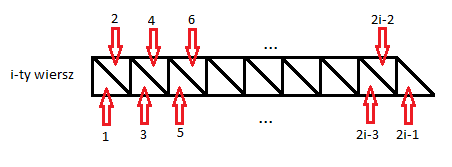
\includegraphics[]{images/division-row.png}
		\caption{Podział $i$-tego wiersza}
		\label{division-row}
	\end{figure}

	Niech $P_0, P_1, P_2$ będą współrzędnymi wierzchołków trójkąta przed podziałem zdefiniowanym analogicznie jak na rysunku \ref{D-area}. Podział na wiersze rozpoczynamy od $P_2$, zatem trójkąt po podziale, którego jednym z wierzchołków będzie $P_2$ znajdzie się w pierwszym wierszu.
	
	Zdefiniujmy następujące zmienne:
	\begin{align*}
		h_x & = \frac{P_1 - P_0}{n} \\
		h_y & = \frac{P_0 - P_2}{n}
	\end{align*}
	Wtedy $h_x$ będzie wektorem, o jaki należy się przesunąć, aby uzyskać współrzędne kolejnej kolumny, natomiast $h_y$ będzie wektorem, o jaki należy się przesunąć, aby uzyskać współrzędne kolejnego wiersza. Zakładam, że każda kolumna oprócz ostatniej w danym wierszu posiada 2 trójkąty.
	
	Zatem jeżeli trójkąt ma nieparzysty indeks, to znajduje się bliżej kolejnego wiersza ("na dole"), a te z indeksem parzystym są bliżej poprzedniego wiersza ("na górze"), jak na rysunku \ref{division-row}.
	
	Aby wyznaczyć współrzędne trójkąta o indeksach $(i, j)$, gdzie $i \in \{1, 2, \dots, n\}$, $j \in \{1, 2, \dots, 2i-1\}$, w oparciu o współrzędne wierzchołka $P_2$ należy rozważyć dwa przypadki:
	
	\begin{enumerate}[label=\textbf{\Roman*}]
		\item $2 \mid j$
		
		\begin{figure}[H]
			\centering
			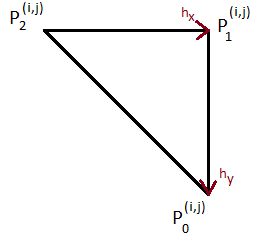
\includegraphics[]{images/triangle-j-even.png}
			\caption{Trójkąt po podziale, gdy $j$ - parzyste}
			\label{triangle-j-even}
		\end{figure}
		
		Wtedy
		\begin{align*}
			P_2^{(i,j)} & = P_2 + (i-1)h_y + \frac{j-2}{2}h_x \\
			P_1^{(i,j)} & = P_2^{(i,j)} + h_x                 \\
			P_0^{(i,j)} & = P_1^{(i,j)} + h_y
		\end{align*}
		
		
		\pagebreak
		
		\item $2 \centernot\mid j$
		
		\begin{figure}[H]
			\centering
			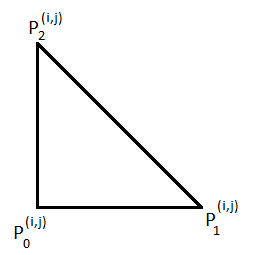
\includegraphics[]{images/triangle-j-odd.png}
			\caption{Trójkąt po podziale, gdy $j$ - nieparzyste}
			\label{triangle-j-odd}
		\end{figure}
		
		Wtedy
		\begin{align*}
			P_2^{(i,j)} & = P_2 + (i-1)h_y + \frac{j-1}{2}h_x \\
			P_0^{(i,j)} & = P_2^{(i,j)} + h_y                 \\
			P_1^{(i,j)} & = P_0^{(i,j)} + h_x
		\end{align*}
	\end{enumerate}
	gdzie $P_k^{(i,j)}$ oznacza współrzędne k-tego wierzchołka trójkąta o indeksach $(i, j)$ po podziale (analogicznie do rysunków w podpunktach).
	
	
	
	
	
	\section{Implementacja metody}
	Metoda zaimplementowana jest na podstawie czterech funkcji oraz jednego skryptu pozwalającego na łatwe jej wykorzystanie i porównanie z funkcją \textit{integral2} z MATLABa:
	\begin{itemize}
		\item $[h_x, h_y, P] = computeDivisionProperties(P_0, P_1, P_2, n)$
		
		Funkcja oblicza własności podziału trójkąta o wierzchołkach $P_0, P_1, P_2$ na $n^2$ trójkątów przystających (zgodnie z powyższym opisem metody). Zwraca wektory $h_x, h_y$ oraz pole trójkąta $P$ po podziale.
		
		
		\item $[P_0^{(i,j)}, P_1^{(i,j)}, P_2{(i,j)}] = computeSingleTriangleCoordinates(P_2, h_x, h_y, i, j)$
		
		Funkcja oblicza współrzędne trójkąta o indeksie $(i, j)$ po podziale na podstawie współrzędnej $P_2$ trójkąta przed podziałem oraz wektorów $h_x, h_j$.
		
		\item $nodeValues = tabulateIntegrationNodeValues(f, P_2, n, h_x, h_y)$
		
		Funkcja tablicuje wartości w wierzchołkach oraz środkach boków trójkątów w celu późniejszego wielokrotnego wykorzystania. Jest to rozwiązanie bardziej efektywne niż obliczanie tych wartości każdorazowo dla poszczególnych trójkątów. Korzysta z wcześniej obliczonych parametrów $h_x$, $h_y$, ilości podziałów $n$ oraz współrzędnej $P_2$ trójkąta, na którym stosowana jest kwadratura. Zwraca macierz rozmiaru $2n+1 \times 2n+1$.
		
		Powiązanie wartości z tej macierzy z współrzędnymi trójkąta zostało zilustrowane na rysunku \ref{triangle-nodes}.
		
		\begin{figure}[H]
			\centering
			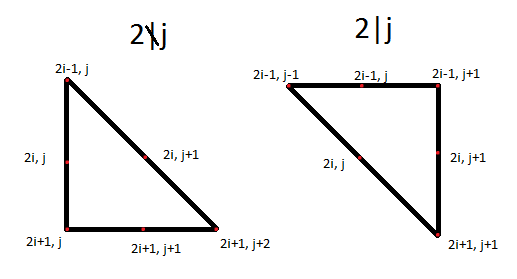
\includegraphics[]{images/triangle-nodes.png}
			\caption{Indeksy w stablicowanej macierzy dla trójkąta o indeksach ($i$, $j$)}
			\label{triangle-nodes}
		\end{figure}
		
		
		\item $S = integrateSingleTriangle(f, P_0, P_1, P_2, P, i, j, nodeValues)$
		
		Funkcja przybliża wartość całki z funkcji podcałkowej $f$ na trójkącie o polu $P$ i wierzchołkach $P_0, P_1, P_2$, używając do tego kwadratury \eqref{kwadratura}. Trójkąt znajduje się na $j$-tej pozycji w $i$-tym wierszu podziału. Stablicowane wartości funkcji są przekazane w macierzy $nodeValues$ (jest to macierz zwrócona przez funkcję $tabulateIntegrationNodeValues$).
		
		
		\item $S = numericalIntegrationTriangle(f, P_0, P_1, P_2, n)$
		
		Funkcja przybliża wartość całki z funkcji podcałkowej $f$ na trójkącie o wierzchołkach $P_0, P_1, P_2$, dzieląc go na $n^2$ trójkątów przystających.
		
		Funkcja używa $computeDivisionProperties$ do uzyskania własności podziału ($h_x, h_y, P$), a następnie wykonuje przybliżenie całki na każdym z trójkątów po podziale używając funkcji $computeSingleTriangleCoordinates$ do uzyskania współrzędnych tego trójkąta, oraz $integrateSingleTriangle$ do uzyskania wartości kwadratury.
		
		\item $integrateDiamond$
		
		Skrypt pozwalający określić funkcję podcałkową $f$ oraz parametr $n$ określający liczbę podziałów. Wykonuje zadanie - przybliża całkę na obszarze $D$ (rysunek \ref{D-area}).
		
		Skrypt dodatkowo podaje informacje o szybkości działania metody oraz porównuje ją z funkcją $integral2$ dostępną w MATLABie.
	\end{itemize}

	Funkcji można używać do przybliżania całki na dowolnym trójkącie, zatem nie musi być to romb podzielony na 4 trójkąty. Wystarczy zmodyfikować skrypt $integrateDiamond$.
	
	Nie jest to jednak tematem zadania, więc postanowiono zostawić to jako zadanie dla ciekawego czytelnika.
	
	
	
	
	\section{Poprawność metody}
	Kwadratura \eqref{kwadratura} jest rzędu 4, zatem dla wielomianów stopnia co najwyżej 3 metoda daje poprawne wyniki, nawet z $n = 1$. Dla wielomianów stopnia wyższego przybliżenie nie jest dokładne, ale dokładność wzrasta wraz ze wzrostem parametru $n$.
	
	
	
	
	\section{Przykłady}
	W przykładach najpierw została obliczona prawdziwa wartość całki, a następnie porównane w tabeli wyniki metody z zadania oraz funkcji \textit{integral2}.
	
	\begin{enumerate}[label=\textbf{Przykład \arabic*}]
		\item
		Całka z wielomianu stopnia 3.
		$$\iint_D f(x, y) \,dx\,dy = \iint_D x^3 \,dx\,dy = 0$$
		$n = 1$
		
		\begin{table}[H]
			\centering
			\begin{tabular}{|r|c|c|}
				\hline
				                   & metoda z zadania & funkcja \textit{integral2} \\ \hline
				przybliżenie całki &        0         & $1.47451 \times 10^{-17}$  \\ \hline
				   czas obliczania &      2.6 ms      &          4.13 ms           \\ \hline
			\end{tabular}
		\end{table}
	
		Metoda z zadania jest dokładna (i powinna być, gdyż rząd kwadratury jest równy 4, a funkcja podcałkowa jest wielomianem stopnia 3), a także szybsza.
		
		
		
		\item
		Całka z wielomianu stopnia 4.
		$$\iint_D f(x, y) \,dx\,dy = \iint_D x^4 \,dx\,dy = \frac{2}{15} \approx 0.133333$$
		$n = 1$
		
		\begin{table}[H]
			\centering
			\begin{tabular}{|r|c|c|}
				\hline
				                   & metoda z zadania & funkcja \textit{integral2} \\ \hline
				przybliżenie całki &     0.144444     &          0.133333          \\ \hline
				   czas obliczania &     6.19 ms      &           4.7 ms           \\ \hline
			\end{tabular}
		\end{table}
	
		W tym przypadku metoda z zadania okazała się gorsza od funkcji dostępnej w MATLABie, zarówno pod względem dokładności, jak i szybkości działania.
		
		
		\item
		Zwiększenie parametru $n$ w stosunku do poprzedniego przykładu.
		$$\iint_D f(x, y) \,dx\,dy = \iint_D x^4 \,dx\,dy = \frac{2}{15} \approx 0.133333$$
		$n = 10$
		
		\begin{table}[H]
			\centering
			\begin{tabular}{|r|c|c|}
				\hline
				                   & metoda z zadania & funkcja \textit{integral2} \\ \hline
				przybliżenie całki &     0.133334     &          0.133333          \\ \hline
				   czas obliczania &     16.34 ms     &          6.06 ms           \\ \hline
			\end{tabular}
		\end{table}
	
		Przy zwiększeniu ilości podziałów metoda osiąga lepsza dokładność, jednakże zmniejsza się jej szybkość. W tym przypadku nadal jest gorsza od funkcji \textit{integral2}.
		
		Podobną dokładność osiąga dopiero dla $n = 17$, jednakże wtedy jej czas działania około dziesięciokrotnie większy od MATLABowej alternatywy.
		
		
		\item
		Funkcja podcałkowa nie będąca wielomianem.
		$$\iint_D f(x, y) \,dx\,dy = \iint_D (\sin x + \cos y) \,dx\,dy = 4 - 4\cos 1 \approx 1.83879$$
		$n = 1$
		
		\begin{table}[H]
			\centering
			\begin{tabular}{|r|c|c|}
				\hline
				                   & metoda z zadania & funkcja \textit{integral2} \\ \hline
				przybliżenie całki &      1.8392      &          1.83879           \\ \hline
				   czas obliczania &     3.36 ms      &           2.9 ms           \\ \hline
			\end{tabular}
		\end{table}
		
		Po raz kolejny funkcja dostępna w MATLABie jest szybsza i dokładniejsza.
		
		Dla $n = 4$ metoda z zadania osiąga podobną dokładność.
		\begin{table}[H]
			\centering
			\begin{tabular}{|r|c|c|}
				\hline
				                   & metoda z zadania & funkcja \textit{integral2} \\ \hline
				przybliżenie całki &     1.83879      &          1.83879           \\ \hline
				   czas obliczania &     4.66 ms      &          3.13 ms           \\ \hline
			\end{tabular}
		\end{table}
	
	
	
		\item
		Wielomian stopnia 7.
		$$\iint_D f(x, y) \,dx\,dy = \iint_D (x^7 + x^6 + y^4 + y^3) \,dx\,dy = \frac{43}{210} \approx 0.204762$$
		$n = 1$
		
		\begin{table}[H]
			\centering
			\begin{tabular}{|r|c|c|}
				\hline
				                   & metoda z zadania & funkcja \textit{integral2} \\ \hline
				przybliżenie całki &     0.254012     & 0.204762                   \\ \hline
				   czas obliczania &     3.59 ms      & 6.96 ms                    \\ \hline
			\end{tabular}
		\end{table}
	
		W tym przypadku metoda z zadania okazała się być szybsza, ale nie dokładniejsza. Podobną dokładność osiąga dla $n = 16$:
		
		\begin{table}[H]
			\centering
			\begin{tabular}{|r|c|c|}
				\hline
				                   & metoda z zadania & funkcja \textit{integral2} \\ \hline
				przybliżenie całki &     0.204762     & 0.204762                   \\ \hline
				   czas obliczania &     40.65 ms     & 7.05 ms                    \\ \hline
			\end{tabular}
		\end{table}
		
	\end{enumerate}
	
	
	
	
	
	
	\section{Wnioski}
	\begin{enumerate}
		\item Czas działania wzrasta kwadratowo wraz ze wzrostem parametru $n$.
		
		\item Metoda z zadania osiąga gorsze wyniki od funkcji \textit{integral2} dostępnej w MATLABie. Jest w stanie osiągnąć podobną dokładność, jednak kosztem znacznego zwiększenia się czasu potrzebnego na obliczenia.
		
		\item Jeżeli nie zależy nam na dokładności, można użyć metody z zadania z $n = 1$, wtedy jest bardzo prawdopodobnym, że będzie ona szybsza od funkcji \textit{integral2}.
	\end{enumerate}

	
	
	
	
	
	\section{Skrypt do testowania}
	Skrypt \textit{integrateDiamond} pozwala na ustalanie funkcji podcałkowej $f$ oraz parametru $n$ określającego ilość podziałów obszaru $D$. Wyświetla on także czas przybliżania całki tą metodą oraz porównuje wyniki z funkcją \textit{integral2} dostępną w MATLABie.
	
	Skrypt zgodnie z opisem metody dzieli obszar $D$ na 4 trójkąty przystające, a następnie każdy z nich na $n^2$ trójkątów przystających i na nich stosuje kwadraturę.
	
	Pokazuje on także jak używać funkcji stworzonych na potrzeby tej metody do przybliżania całki na dowolnym trójkącie.
	
	\begin{lstlisting}[frame=single]
	% Parametry:
	% Funkcja podcalkowa
	f = @(x, y)(x.^2 + y.^2);
	% Liczba okreslajaca ilosc podzialow
	n = 1;
	
	% Srodek rombu
	P0 = [0 0];
	% Wierzcholki rombu
	P1 = [1 0];
	P2 = [0 1];
	P3 = [-1 0];
	P4 = [0 -1];
	
	% Kwadratura dla trojkatow w poszczegolnych cwiartkach ukladu wspolrzednych
	S1 = numericalIntegrationTriangle(f, P0, P1, P2, n); % I cwiartka
	S2 = numericalIntegrationTriangle(f, P0, P2, P3, n); % II cwiartka
	S3 = numericalIntegrationTriangle(f, P0, P3, P4, n); % III cwiartka
	S4 = numericalIntegrationTriangle(f, P0, P4, P1, n); % IV cwiartka
	
	S = S1 + S2 + S3 + S4;
	\end{lstlisting}
	
	
	
	\section{Bibliografia}
	\begin{enumerate}
		\item Informacje z wykładu \textit{Metod numerycznych 2} (wydział MiNI PW, dr Iwona Wróbel) (w szczególności wzór na kwadraturę rzędu 4 na trójkącie)
	\end{enumerate}
	
\end{document}